\section{Basic System Design}

We use the same system design presented by PacketShader and Gnort. Pictured in
Figure~\ref{fig:system}, packets pass through our system as follows: (1) As
packets arrive at the NIC, they are copied to main memory via DMA. (2) Software
running on the CPU copies these new packets to a buffer until (3) a sufficient
number have arrived (see below) and the batch is transferred to memory on the
GPU. (4) The GPU processes the packets in parallel and fills a buffer of
results on the GPU which (5) the CPU copies back to main memory when processing
has finished. (6) Using these results, the CPU instructs the NIC(s) where to
forward each packet in the batch; (7) finally, the NIC(s) fetch(es) the packets
from main memory with another DMA and forwards them.

\begin{figure}
   \centering
   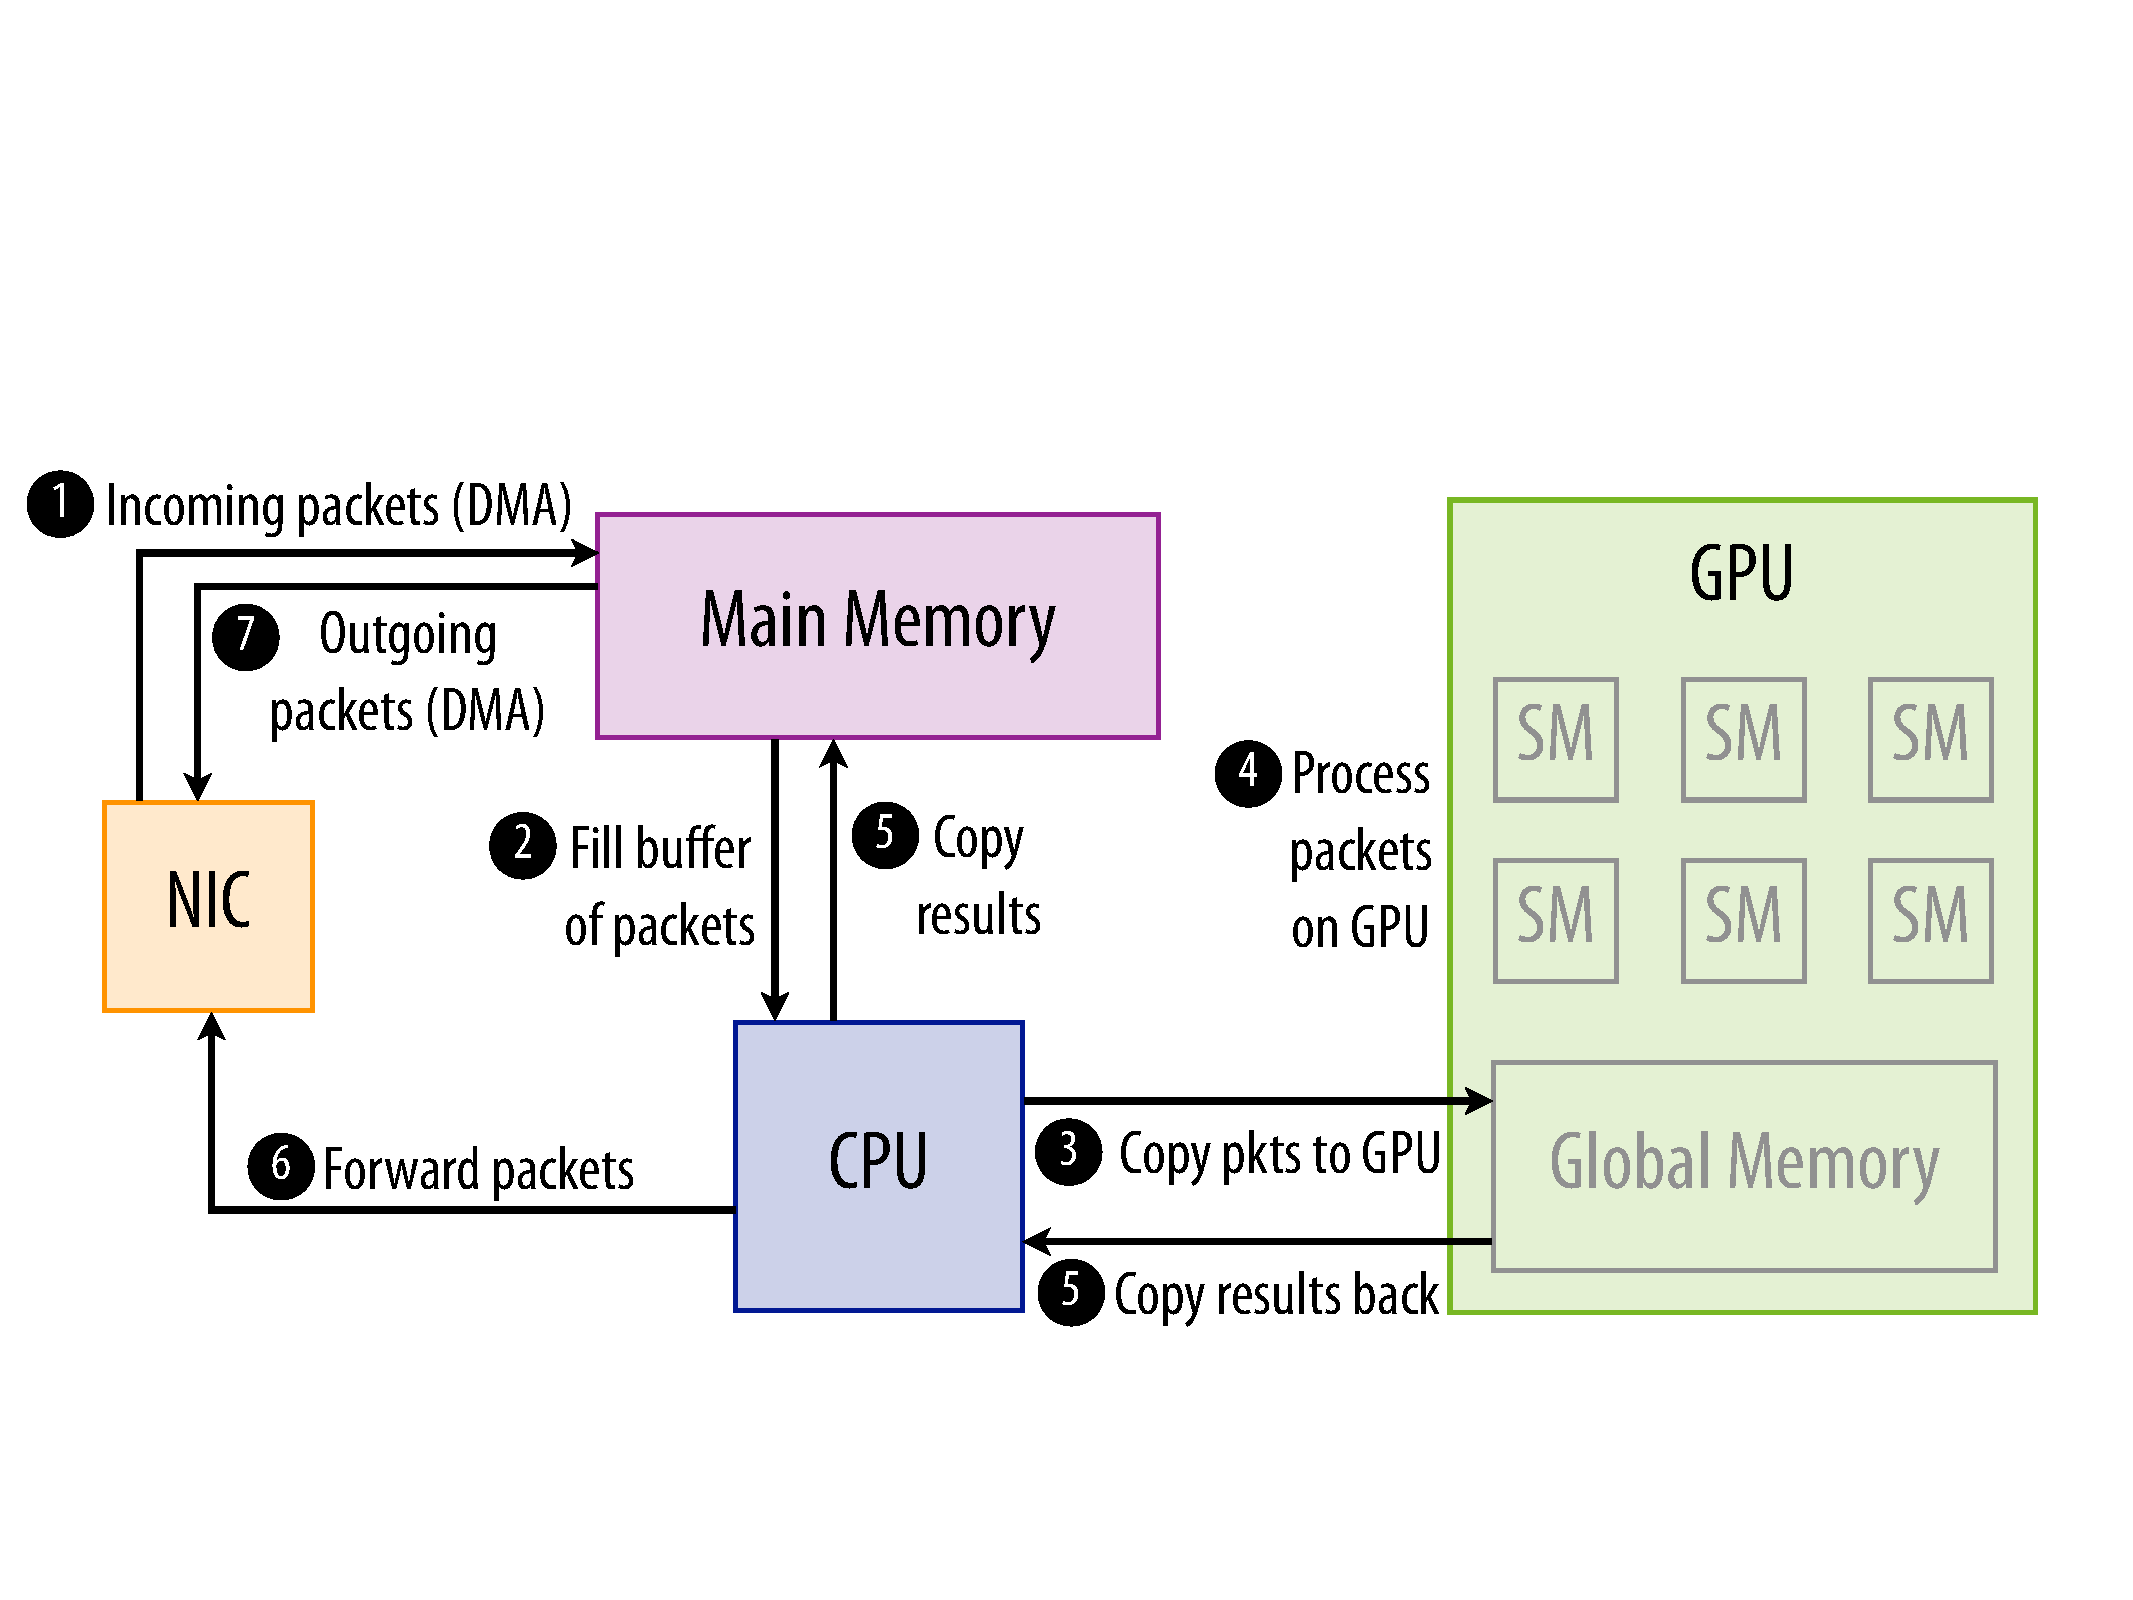
\includegraphics[scale=0.23]{figs/system_overview.pdf} 
   \caption{Basic System Design}
   \label{fig:system}
\end{figure}

\subsection{GPU Programming Issues}
\noindent \textbf{Pipelining.} As with almost any CUDA program, ours employs
pipelining for data transfers between main memory and GPU memory. While the GPU
is busy processing a batch of packets, we can utilize the CPU to copy the
results from the previous batch of packets from the GPU back to main memory and
copy the next batch of packets to the GPU (Figure~\ref{fig:pipelining}). In
this way, we never let CPU cycles go idle while the GPU is working.\\

\begin{figure}
   \centering
   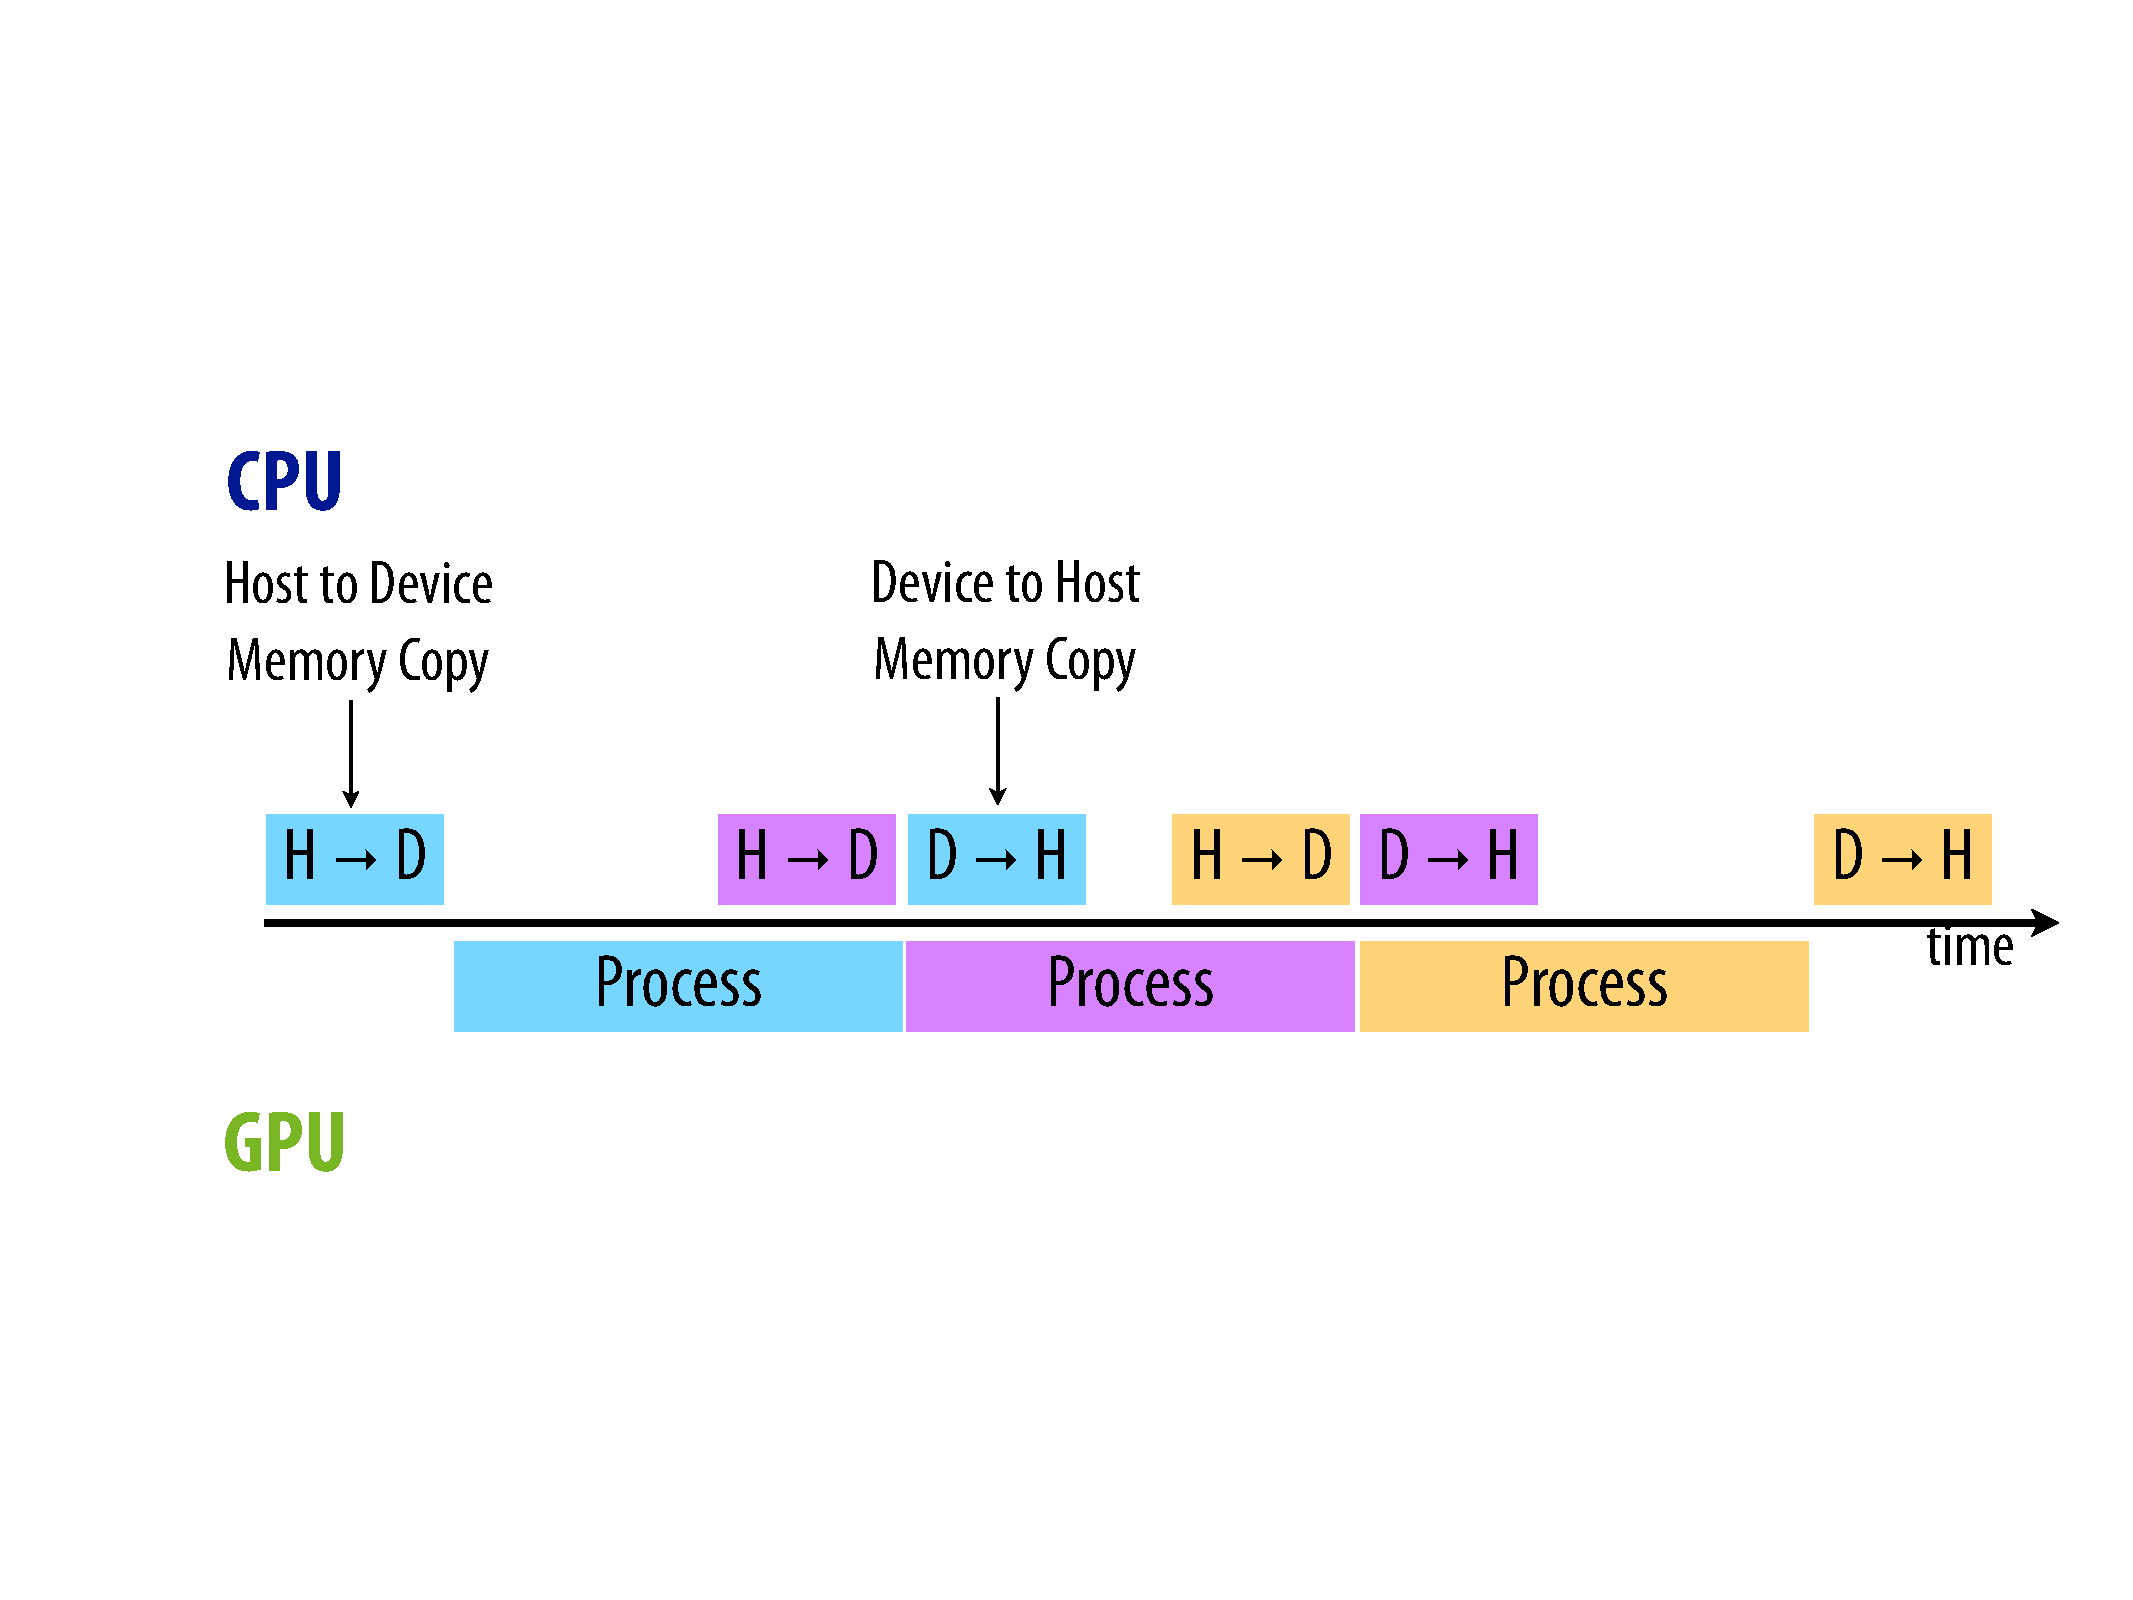
\includegraphics[scale=0.25]{figs/pipelining.pdf}
   \caption{Pipelined Execution}
   \label{fig:pipelining}
\end{figure}

\noindent \textbf{Batching.} Although the GPU can process hundreds of packets
in parallel (unlike the CPU), there is, of course, a cost: non-trivial overhead
is incurred in transferring packets to the GPU and copying results back from
it. To amortize this cost, we process packets in batches...

\subsection{Packet Processing}

\subsubsection{Longest Prefix Match}

\subsubsection{Firewall Rule Matching}
